\documentclass[a4paper]{article}
\usepackage[a4paper]{geometry}
%\usepackage{fullpage}
\usepackage{fancyhdr}
\usepackage[english,francais]{babel}
\usepackage[T1]{fontenc}
\usepackage[utf8]{inputenc}
\usepackage[pdftex]{graphicx}
\usepackage{subfig}
\usepackage{hyperref}
%\usepackage{hyperref}

%\renewcommand{\baselinestretch}{2}
\author{Danchi \textsc{Li} \and Florent \textsc{Guiotte}}
\title{Eigenfaces \\ \Large{Compte rendu de résultats}}
\pagestyle{fancy}

\begin{document}
\maketitle
\tableofcontents

\section{Introduction}

L'objectif de ce projet est de développer un système de reconnaissance de visages à l'aide des {\em eigenfaces}.
Nous utilisons une base de donnée de visage issue de l'{\em Olivetti Research Laboratory}
que nous avons divisé en deux ensembles, de référence et de test.

Ce rapport étudie les propriétés de la méthode de reconnaissance des visages avec des eigenfaces et les résultats
que nous avons obtenus.

\section{Mise en pratique}

Pour réaliser ce projet, nous avons utilisé~:
\begin{itemize}
    \item ViSP 3.0.1
    \item CMake 3.4.3
\end{itemize}

\subsection{Question 1}

La taille de la mémoire nécessaire pour stocker une image I sous la forme d'une matrice de réels (avec une 
précision de {\em double} soit 64 bit par élément) est de~:
\[
    M_m = h \times l \times 8
\]
Où $M_m$ est la taille d'une image exprimée en octet et avec $h$ et $l$ représentant respectivement la hauteur
et la largeur d'une image $I_m$.
\[
    M_I = M_m \times n
\]
Où $M_I$ est la taille de la matrice $I$ exprimée en octet et $n$ le nombre d'images dans la base de données.
Dans notre cas <<au plus>>, avec des images de taille $92 \times 112$ et avec 400 images dans la base de
données, la matrice occupe une place de 33Mo en mémoire.

\subsection{Question 2 et 3}

Nous calculons le visage moyen $\Psi$ à l'aide de la méthode {\em initMeanFace} dans la classe {\em
Eigenfaces.h}. Il s'agit de la composante de base de nos eigenfaces. Notre résultat est visible figure
\ref{q3a:mean_face}.
\begin{figure}%[!ht]%htp]
  \centering
  \subfloat[Visage moyen $\Psi$]{\label{q3a:mean_face}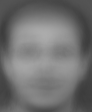
\includegraphics{img/mean_face.png}}
  \hspace{0.01\textwidth}
  \subfloat[Visage du sujet 1]{\label{q3a:face_s1}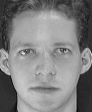
\includegraphics{img/q3_face_s1.png}}
  \hspace{0.01\textwidth}
  \subfloat[Visage centré]{\label{q3a:center_s1}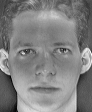
\includegraphics{img/q3_center_s1.png}}
  \\
  \subfloat[Visage moyen $\Psi$]{\label{q3a:mean_face2}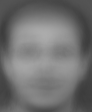
\includegraphics{img/mean_face.png}}
  \hspace{0.01\textwidth}
  \subfloat[Visage du sujet 10]{\label{q3a:face_s10}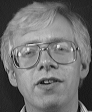
\includegraphics{img/q3_face_s10.png}}
  \hspace{0.01\textwidth}
  \subfloat[Visage centré]{\label{q3a:center_s10}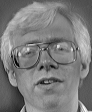
\includegraphics{img/q3_center_s10.png}}
  \\
  \subfloat[Visage moyen $\Psi$]{\label{q3a:mean_face3}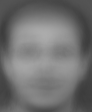
\includegraphics{img/mean_face.png}}
  \hspace{0.01\textwidth}
  \subfloat[Visage du sujet 20]{\label{q3a:face_s20}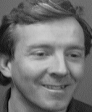
\includegraphics{img/q3_face_s20.png}}
  \hspace{0.01\textwidth}
  \subfloat[Visage centré]{\label{q3a:center_s20}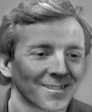
\includegraphics{img/q3_center_s20.png}}
  \\
  \caption{Affichage du visage moyen et de visages centrés}
  \label{q3a}
\end{figure}

\section{Analyse en composantes principales}

\subsection{Question 4 et 5}

La matrice $U$ représente les vecteurs propres de la matrice de covarience $A.A^T$, où 
$A = [I_1 - \Psi ... I_m - \Psi]$.
Cette matrice correspond donc aux eigenfaces.

Nous avons calculé cette matrice $U$ à l'aide de la méthode {\em computeEigenfaces} de la classe {\em
Eigenfaces.h}. Cette méthode utilise la {\em singular value decomposition (SVD)} sur la matrice $A$ pour
obtenir des valeurs singulières plutôt que des valeurs propres.

\subsection{Question 6}

Nous avons utilisé 9 visages sur 10 par sujet, avec 36 sujets pour construire notre matrice des eigenfaces.
Le reste des images -- 1 visage par sujet déjà présents dans la base plus 10 visages chez 4 sujets n'étant pas du tout
présents dans $A$ lors la construction de la matrice des eigenfaces -- nous servent de données de test.
Nous avons affichés les sept premières eigenfaces. Nos résultats sont visibles figure \ref{q6}.

\begin{figure}%[!ht]%htp]
  \centering
  \subfloat[Visage moyen $\Psi$]{\label{q6:mean_face}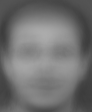
\includegraphics{img/mean_face.png}}
  \hspace{0.01\textwidth}
  \subfloat[Eigenface 1]{\label{q6:ef1}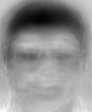
\includegraphics{img/q6_eigenface_1.png}}
  \hspace{0.01\textwidth}
  \subfloat[Eigenface 2]{\label{q6:ef2}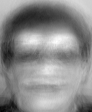
\includegraphics{img/q6_eigenface_2.png}}
  \hspace{0.01\textwidth}
  \subfloat[Eigenface 3]{\label{q6:ef3}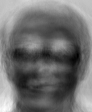
\includegraphics{img/q6_eigenface_3.png}}
  \hspace{0.01\textwidth}
  \subfloat[Eigenface 4]{\label{q6:ef4}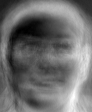
\includegraphics{img/q6_eigenface_4.png}}
  \hspace{0.01\textwidth}
  \subfloat[Eigenface 5]{\label{q6:ef5}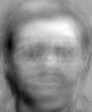
\includegraphics{img/q6_eigenface_5.png}}
  \hspace{0.01\textwidth}
  \subfloat[Eigenface 6]{\label{q6:ef6}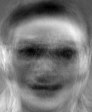
\includegraphics{img/q6_eigenface_6.png}}
  \hspace{0.01\textwidth}
  \subfloat[Eigenface 7]{\label{q6:ef7}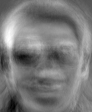
\includegraphics{img/q6_eigenface_7.png}}
  \hspace{0.01\textwidth}
  \caption{Affichage des premières eigenfaces}
  \label{q6}
\end{figure}

\section{Projection dans le sous-espace des visages}

\subsection{Question 7}

Nous calculons les coordonnées des visages de référence et de tests dans le sous-espace des visages à l'aide
de la méthode {\em getFaceCoordinates} de la classe {\em Eigenfaces.h}.
À partir de ces coordonnées nous pouvons reconstruire en une image correspondante à l'aide de la méthode 
{\em getFaceWithCoordinates}.

\subsection{Question 8}

Nous affichons les résultats de ces reconstruction en faisant varier le paramètre $K$ qui permet de déterminer
le nombre d'eigenface à prendre en compte lors de la transformation dans le sous-espace.
Le vecteur de coordonnée est donc de taille $K$. L'organisation de la matrice $U$ lors de la SVD concentre les
informations importantes dans les premières eigenfaces 
-- ce qui est un résultat semblable à la concentration des basses fréquence lors d'une DCT -- 
ce qui nous permet de transmettre le maximum d'informations possible pour un $K$ donné.

Les résultats de nos reconstructions sont divisés en trois classes~:
\begin{itemize}
    \item La première classe (figure \ref{q8c1}) correspond aux visages présents dans la matrice $I$ ayant servit à la construction des
        eigenfaces.
    \item La deuxième classe (figure \ref{q8c2}) correspond à des visages non présents dans la matrice $I$ mais
        dont le sujet à déjà plusieurs autre visages référencés dans $I$.
    \item La troisième classe (figure \ref{q8c3}) correspond à des visages de sujet totalement inconnus de la
        matrice $I$.
\end{itemize}

\begin{figure}[!ht]%htp]
  \centering
  \subfloat[s1i1]{\label{q8:s1i1}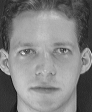
\includegraphics[width=0.09\textwidth]{img/q8r_1_1.png}}
  \hspace{0.001\textwidth}
  \subfloat[1]{\label{q8:s1i1k1}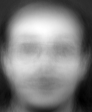
\includegraphics[width=0.09\textwidth]{img/q8r_1_1_k1.png}}
  \hspace{0.001\textwidth}
  \subfloat[5]{\label{q8:s1i1k5}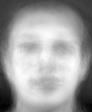
\includegraphics[width=0.09\textwidth]{img/q8r_1_1_k5.png}}
  \hspace{0.001\textwidth}
  \subfloat[10]{\label{q8:s1i1k10}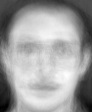
\includegraphics[width=0.09\textwidth]{img/q8r_1_1_k10.png}}
  \hspace{0.001\textwidth}
  \subfloat[30]{\label{q8:s1i1k30}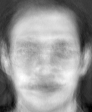
\includegraphics[width=0.09\textwidth]{img/q8r_1_1_k30.png}}
  \hspace{0.001\textwidth}
  \subfloat[50]{\label{q8:s1i1k50}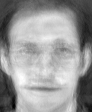
\includegraphics[width=0.09\textwidth]{img/q8r_1_1_k50.png}}
  \hspace{0.001\textwidth}
  \subfloat[100]{\label{q8:s1i1k100}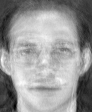
\includegraphics[width=0.09\textwidth]{img/q8r_1_1_k100.png}}
  \hspace{0.001\textwidth}
  \subfloat[200]{\label{q8:s1i1k200}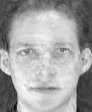
\includegraphics[width=0.09\textwidth]{img/q8r_1_1_k200.png}}
  \hspace{0.001\textwidth}
  \subfloat[300]{\label{q8:s1i1k300}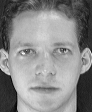
\includegraphics[width=0.09\textwidth]{img/q8r_1_1_k300.png}}
  \hspace{0.001\textwidth}
  \subfloat[324]{\label{q8:s1i1k324}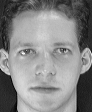
\includegraphics[width=0.09\textwidth]{img/q8r_1_1_k324.png}}
  \\
  \subfloat[s10i1]{\label{q8:s10i1}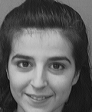
\includegraphics[width=0.09\textwidth]{img/q8r_10_1.png}}
  \hspace{0.001\textwidth}
  \subfloat[1]{\label{q8:s10i1k1}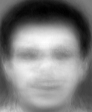
\includegraphics[width=0.09\textwidth]{img/q8r_10_1_k1.png}}
  \hspace{0.001\textwidth}
  \subfloat[5]{\label{q8:s10i1k5}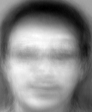
\includegraphics[width=0.09\textwidth]{img/q8r_10_1_k5.png}}
  \hspace{0.001\textwidth}
  \subfloat[10]{\label{q8:s10i1k10}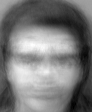
\includegraphics[width=0.09\textwidth]{img/q8r_10_1_k10.png}}
  \hspace{0.001\textwidth}
  \subfloat[30]{\label{q8:s10i1k30}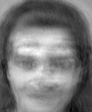
\includegraphics[width=0.09\textwidth]{img/q8r_10_1_k30.png}}
  \hspace{0.001\textwidth}
  \subfloat[50]{\label{q8:s10i1k50}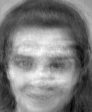
\includegraphics[width=0.09\textwidth]{img/q8r_10_1_k50.png}}
  \hspace{0.001\textwidth}
  \subfloat[100]{\label{q8:s10i1k100}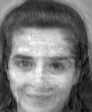
\includegraphics[width=0.09\textwidth]{img/q8r_10_1_k100.png}}
  \hspace{0.001\textwidth}
  \subfloat[200]{\label{q8:s10i1k200}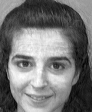
\includegraphics[width=0.09\textwidth]{img/q8r_10_1_k200.png}}
  \hspace{0.001\textwidth}
  \subfloat[300]{\label{q8:s10i1k300}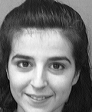
\includegraphics[width=0.09\textwidth]{img/q8r_10_1_k300.png}}
  \hspace{0.001\textwidth}
  \subfloat[324]{\label{q8:s10i1k324}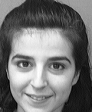
\includegraphics[width=0.09\textwidth]{img/q8r_10_1_k324.png}}
  \caption{Reconstruction de visage de la première classe en fonction de $K$}
  \label{q8c1}
\end{figure}

\begin{figure}[!ht]%htp]
  \centering
  \subfloat[s1i10]{\label{q8:s1i10}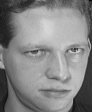
\includegraphics[width=0.09\textwidth]{img/q8r_1_10.png}}
  \hspace{0.001\textwidth}
  \subfloat[1]{\label{q8:s1i10k1}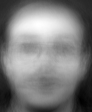
\includegraphics[width=0.09\textwidth]{img/q8r_1_10_k1.png}}
  \hspace{0.001\textwidth}
  \subfloat[5]{\label{q8:s1i10k5}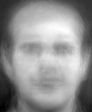
\includegraphics[width=0.09\textwidth]{img/q8r_1_10_k5.png}}
  \hspace{0.001\textwidth}
  \subfloat[10]{\label{q8:s1i10k10}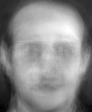
\includegraphics[width=0.09\textwidth]{img/q8r_1_10_k10.png}}
  \hspace{0.001\textwidth}
  \subfloat[30]{\label{q8:s1i10k30}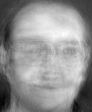
\includegraphics[width=0.09\textwidth]{img/q8r_1_10_k30.png}}
  \hspace{0.001\textwidth}
  \subfloat[50]{\label{q8:s1i10k50}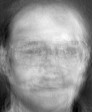
\includegraphics[width=0.09\textwidth]{img/q8r_1_10_k50.png}}
  \hspace{0.001\textwidth}
  \subfloat[100]{\label{q8:s1i10k100}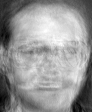
\includegraphics[width=0.09\textwidth]{img/q8r_1_10_k100.png}}
  \hspace{0.001\textwidth}
  \subfloat[200]{\label{q8:s1i10k200}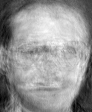
\includegraphics[width=0.09\textwidth]{img/q8r_1_10_k200.png}}
  \hspace{0.001\textwidth}
  \subfloat[300]{\label{q8:s1i10k300}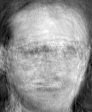
\includegraphics[width=0.09\textwidth]{img/q8r_1_10_k300.png}}
  \hspace{0.001\textwidth}
  \subfloat[324]{\label{q8:s1i10k324}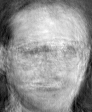
\includegraphics[width=0.09\textwidth]{img/q8r_1_10_k324.png}}
  \\
  \subfloat[s10i10]{\label{q8:s10i10}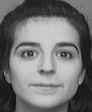
\includegraphics[width=0.09\textwidth]{img/q8r_10_10.png}}
  \hspace{0.001\textwidth}
  \subfloat[1]{\label{q8:s10i10k1}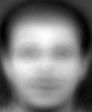
\includegraphics[width=0.09\textwidth]{img/q8r_10_10_k1.png}}
  \hspace{0.001\textwidth}
  \subfloat[5]{\label{q8:s10i10k5}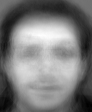
\includegraphics[width=0.09\textwidth]{img/q8r_10_10_k5.png}}
  \hspace{0.001\textwidth}
  \subfloat[10]{\label{q8:s10i10k10}\includegraphics[width=0.09\textwidth]{img/q8r_10_10_k10.png}}
  \hspace{0.001\textwidth}
  \subfloat[30]{\label{q8:s10i10k30}\includegraphics[width=0.09\textwidth]{img/q8r_10_10_k30.png}}
  \hspace{0.001\textwidth}
  \subfloat[50]{\label{q8:s10i10k50}\includegraphics[width=0.09\textwidth]{img/q8r_10_10_k50.png}}
  \hspace{0.001\textwidth}
  \subfloat[100]{\label{q8:s10i10k100}\includegraphics[width=0.09\textwidth]{img/q8r_10_10_k100.png}}
  \hspace{0.001\textwidth}
  \subfloat[200]{\label{q8:s10i10k200}\includegraphics[width=0.09\textwidth]{img/q8r_10_10_k200.png}}
  \hspace{0.001\textwidth}
  \subfloat[300]{\label{q8:s10i10k300}\includegraphics[width=0.09\textwidth]{img/q8r_10_10_k300.png}}
  \hspace{0.001\textwidth}
  \subfloat[324]{\label{q8:s10i10k324}\includegraphics[width=0.09\textwidth]{img/q8r_10_10_k324.png}}
  \caption{Reconstruction de visage de la deuxième classe en fonction de $K$}
  \label{q8c2}
\end{figure}

\begin{figure}[!ht]%htp]
  \centering
  \subfloat[s37i7]{\label{q8:s37i7}\includegraphics[width=0.09\textwidth]{img/q8r_37_7.png}}
  \hspace{0.001\textwidth}
  \subfloat[1]{\label{q8:s37i7k1}\includegraphics[width=0.09\textwidth]{img/q8r_37_7_k1.png}}
  \hspace{0.001\textwidth}
  \subfloat[5]{\label{q8:s37i7k5}\includegraphics[width=0.09\textwidth]{img/q8r_37_7_k5.png}}
  \hspace{0.001\textwidth}
  \subfloat[10]{\label{q8:s37i7k10}\includegraphics[width=0.09\textwidth]{img/q8r_37_7_k10.png}}
  \hspace{0.001\textwidth}
  \subfloat[30]{\label{q8:s37i7k30}\includegraphics[width=0.09\textwidth]{img/q8r_37_7_k30.png}}
  \hspace{0.001\textwidth}
  \subfloat[50]{\label{q8:s37i7k50}\includegraphics[width=0.09\textwidth]{img/q8r_37_7_k50.png}}
  \hspace{0.001\textwidth}
  \subfloat[100]{\label{q8:s37i7k100}\includegraphics[width=0.09\textwidth]{img/q8r_37_7_k100.png}}
  \hspace{0.001\textwidth}
  \subfloat[200]{\label{q8:s37i7k200}\includegraphics[width=0.09\textwidth]{img/q8r_37_7_k200.png}}
  \hspace{0.001\textwidth}
  \subfloat[300]{\label{q8:s37i7k300}\includegraphics[width=0.09\textwidth]{img/q8r_37_7_k300.png}}
  \hspace{0.001\textwidth}
  \subfloat[324]{\label{q8:s37i7k324}\includegraphics[width=0.09\textwidth]{img/q8r_37_7_k324.png}}
  \\
  \subfloat[s40i2]{\label{q8:s40i2}\includegraphics[width=0.09\textwidth]{img/q8r_40_2.png}}
  \hspace{0.001\textwidth}
  \subfloat[1]{\label{q8:s40i2k1}\includegraphics[width=0.09\textwidth]{img/q8r_40_2_k1.png}}
  \hspace{0.001\textwidth}
  \subfloat[5]{\label{q8:s40i2k5}\includegraphics[width=0.09\textwidth]{img/q8r_40_2_k5.png}}
  \hspace{0.001\textwidth}
  \subfloat[10]{\label{q8:s40i2k10}\includegraphics[width=0.09\textwidth]{img/q8r_40_2_k10.png}}
  \hspace{0.001\textwidth}
  \subfloat[30]{\label{q8:s40i2k30}\includegraphics[width=0.09\textwidth]{img/q8r_40_2_k30.png}}
  \hspace{0.001\textwidth}
  \subfloat[50]{\label{q8:s40i2k50}\includegraphics[width=0.09\textwidth]{img/q8r_40_2_k50.png}}
  \hspace{0.001\textwidth}
  \subfloat[100]{\label{q8:s40i2k100}\includegraphics[width=0.09\textwidth]{img/q8r_40_2_k100.png}}
  \hspace{0.001\textwidth}
  \subfloat[200]{\label{q8:s40i2k200}\includegraphics[width=0.09\textwidth]{img/q8r_40_2_k200.png}}
  \hspace{0.001\textwidth}
  \subfloat[300]{\label{q8:s40i2k300}\includegraphics[width=0.09\textwidth]{img/q8r_40_2_k300.png}}
  \hspace{0.001\textwidth}
  \subfloat[324]{\label{q8:s40i2k324}\includegraphics[width=0.09\textwidth]{img/q8r_40_2_k324.png}}
  \caption{Reconstruction de visage de la troisième classe en fonction de $K$}
  \label{q8c3}
\end{figure}

\subsection{Question 9}

Lorsque $K=m$, la reconstruction est parfaite pour les visages de référence. Ces reconstructions sont visibles
pour les visages de la première classe sur les figures \ref{q8:s1i1k324} et \ref{q8:s10i1k324}.

\subsection{Question 10}

On affiche la courbe de la somme cumulée des valeurs propres obtenues avec la SVD. La courbe est visible
figure \ref{q10}.

\begin{figure}
    \centering
    \includegraphics[width=\textwidth]{img/q10_eigen_values.png}
    \caption{Somme cumulée des valeurs propres}
    \label{q10}
\end{figure}

Avec seulement 50 des premières eigenfaces nous obtenons 80\% de l'information contenue dans nos 324
eigenfaces. Et avec les 188 premières, nous avons 97\% de l'information maximum théorique.
Un nombre entre 50 et 200, en fonction de l'utilisation, permet donc d'obtenir une <<bonne>> reconstruction.

\subsection{Question 11}

On trace la courbe d'évolution de la moyenne de l'erreur de reconstruction des visages en faisant varier $K$.
Cette courbe est visible figure \ref{q11}.

\begin{figure}
    \centering
    \includegraphics[width=\textwidth]{img/q11_mean_error.png}
    \caption{Erreur moyenne en fonction de $K$}
    \label{q11}
\end{figure}

Cette évolution est bien cohérente avec la somme cumulée de la question 10, elle affiche une réduction de 
presque 65\% de l'erreur avec $K = 188$.

\section{Identification}

\subsection{Question 12}

Soit la distance entre deux images~:
\[
    E(J) = || J_p - J_p^k ||
\]
Nous pouvons estimer cette distance avec $E_k(J)$ en se limitant à un sous-espace. 
En effet, comme vu précédement, un nombre limité d'eigenfaces permet de représenter une grosse partie de l'information
nécessaire à l'identification.
L'intéret d'utiliser $E_k(J)$ est de gagner du temps de calcul.

\subsection{Question 13}

Nous avons calculé les distances entre toutes les images de références contenues dans $I$.
Pour visualiser ces résultats nous avons affiché une image de matrice visible figure \ref{q13}.

\begin{figure}[!ht]
    \centering
    \includegraphics[width=0.5\textwidth]{img/q13_distance.png}
    \caption{Distance entre les images contenus dans $I$}
    \label{q13}
\end{figure}

L'image se lit de haut en bas et de gauche à droite avec en abscisse et en ordonnée l'indice $m$ de $I_m$.
Plus la luminance est grande, plus l'erreur est élevée. 
On remarque des <<blocs>> d'erreurs faibles sur la diagonale, ce qui correspond à la distance entre les images
d'un même sujet. Ce qui nous permet de valider cette méthode pour l'identification d'un sujet présent dans la
base. Cependant on peut aussi remarquer quelques <<mauvaises>> corrélations entre sujets, ce qui annonce des
faux positifs, et donc le manque de robustesse de cette méthode avec un $K$ faible.

\subsection{Question 14}

Avec $K=20$, concernant la distance entre deux images d'un même sujet nous avons obtenus des distances de
l'ordre de 0.076 en moyenne, 
avec un minimum de 0.010 
-- sans compter les identification d'une même image --
et un maximum de 0.192.
Concernant la distance entre deux images de sujets différents, nous avons obtenus une 
distance moyenne de 0.183 
avec un minimum de 0.011
et un maximum de 0.328.

On peut déjà en déduire que quel que soit le $\theta$ choisi, il y aura des faux positifs.
Nous avons choisi $\theta = 0.100$ ce qui correspond à une identification plutôt stricte.
%Ref. mean error: 0.0764552 min: 0.0102063 max: 0.192549
%Test mean error: 0.1833690 min: 0.0102063 max: 0.328414

\subsection{Question 15}

Nous avons tracé des courbes du nombre de visages reconnus en fonction de $K$ sans modifier $\theta$.
Cette courbe est visible figure \ref{q15}.

\begin{figure}[!ht]
    \centering
    \includegraphics[width=\textwidth]{img/q15_recognition.png}
    \caption{Taux de reconnaissance des visage en fonction de $K$}
    \label{q15}
\end{figure}

La figure se compose de trois courbes~:
\begin{itemize}
    \item La courbe bleu représente le nombre de visages reconnus (Positif).
    \item La courbe rouge représente le nombre de visages non reconnus pourtant appartenant à la même personne
        (Faux-négatif).
    \item La courbe verte représente le nombre de visages faussement reconnus (Faux-positif).
\end{itemize}

Premièrement, ces courbes démontre que nous avons choisi un $\theta$ beaucoup trop strict, dont le choix était
en partie biaisé quand $K=20$.
Cependant, cette courbe permet d'exprimer la tendance de convergence rapide des résultats même avec un $K$
relativement faible. Avec $K=50$ nous devrions avoir une bonne reconnaissance et un temps de calcul correct.

\section{Conclusion}

La méthode des reconnaissance de visages à l'aide des eigenfaces nous permet d'effectuer l'
identification d'un visage connu rapidement, à défaut de réelle robustesse. 
La décomposition en valeurs propres, ou <<visages propres>> nous permet de créer un sous-espace
d'identification permettant d'accélérer énormément les temps de calculs.

\end{document}

%\begin{figure}[!ht]
%    \centering
%    \includegraphics{img/mean_face.png}
%    \caption{Visage moyen $\Psi$}
%    \label{mean_face}
%\end{figure}

%\begin{figure}[!ht]%htp]
%  \centering
%  \subfloat[SURF - knn]{\label{surf:knn}\includegraphics[width=0.49\textwidth]{img/KMeansIndex/knn/corel_0000000303_512_COREL_SURF.jpg}}
%  \hspace{0.01\textwidth}
%  \subfloat[SURF - Spheric]{\label{surf:spheric}\includegraphics[width=0.49\textwidth]{img/KMeansIndex/radius/corel_0000000303_512_COREL_SURF.jpg}}
%  \caption{Résultats avec SURF via une recherche knn (\ref{surf:knn}) et sphérique (\ref{surf:spheric}).}
%  \label{surf}
%\end{figure}
